\documentclass{article}
\usepackage{arxiv}

\usepackage[utf8]{inputenc}
\usepackage[english, russian]{babel}
\usepackage[T1]{fontenc}
\usepackage{url}
\usepackage{booktabs}
\usepackage{amsfonts}
\usepackage{nicefrac}
\usepackage{microtype}
\usepackage{lipsum}
\usepackage{graphicx}
\usepackage{natbib}
\usepackage{doi}
\usepackage{amsmath}
\DeclareMathOperator*{\argmax}{arg\,max}
\DeclareMathOperator*{\softmax}{SoftMax}


\title{Детекция эмоций. Сравнение и анализ классических методов машинного обучения и методов обучения с трансформерами}

\author{ Панин Никита Александрович \\
        Факультет вычислительной математики и кибернетики \\
        МГУ им. Ломоносова \\
        \texttt{s02200456@gse.cs.msu.ru} \\
	%% examples of more authors
	\And
	д.ф-м.н., профессор, Воронцов Константин Вячеславович \\
        Факультет вычислительной математики и кибернетики \\
        МГУ им. Ломоносова \\
        \texttt{vokov@forecsys.ru} \\
	%% \AND
	%% Coauthor \\
	%% Affiliation \\
	%% Address \\
	%% \texttt{email} \\
	%% \And
	%% Coauthor \\
	%% Affiliation \\
	%% Address \\
	%% \texttt{email} \\
	%% \And
	%% Coauthor \\
	%% Affiliation \\
	%% Address \\
	%% \texttt{email} \\
}

\date{}

\renewcommand{\shorttitle}{\textit{arXiv} Template}

%%% Add PDF metadata to help others organize their library
%%% Once the PDF is generated, you can check the metadata with
%%% $ pdfinfo template.pdf
\hypersetup{
pdftitle={Детекция эмоций. Сравнение и анализ классических методов машинного обучения и методов обучения с трансформерами},
pdfsubject={q-bio.NC, q-bio.QM},
pdfauthor={Воронцов Константин Вячеславович,Панин Никита Александрович },
pdfkeywords={},
}

\begin{document}
\maketitle

\begin{abstract}
	В работе была рассмотрена задача детекции эмоций на датасете, в основу которого вошел WASSA датасет из твитов для детекции эмоций. На выходе алгоритма классификации эмоций в твитах была одна из 5 эмоций: нейтральная эмоция, грусть, страх, радость, гнев. Были применены различные методы "классического" машинного обучения, такие как, SVM, логистическая регрессия, метод k-ближайших соседей и наивный байесовский классификатор. Также классификация эмоций была проведена с помощью файн-тюнинга нескольких версий BERT. Основной целью работы являлось проведение сравнительного анализа для классических моделей машинного обучения(wKNN, Multinomial Bayes Classifier, Logistic Regression, SVM) и для моделей глубокого обучения (в качестве предобученной модели брались BERT, RoBERTa, BERTweet и их large-версии). В результате исследования было показано, что по метрике accuracy для моделей классического обучения c tf-idf векторизацией текстов лучше всего работает SVM с RBF ядром ($accuracy \approx 0.8387$ на тесте), а наиболее качественные результаты получаются с помощью предложенной в исследовании модели с предобученным BERTweet ($accuracy \approx 0.88$ на тесте).
\end{abstract}


\keywords{Детекция эмоций \and  NLP}

\section{Введение}
В нашем эмоционально насыщенном мире разумно стремиться к пониманию тонких чувств и настроений, выраженных в текстах. С развитием машинного обучения и искусственного интеллекта, возникает возможность автоматизировать и усовершенствовать процессы анализа и интерпретации текстов, выявляя эмоции, ассоциированные с ними. Детекция эмоций в текстах стала актуальным направлением исследований в области обработки естественного языка (NLP) и анализа тональности и привлекает все большее внимание в последние два десятилетия~\cite{affectdetectionintexts, jiawenfuji}. Термины "распознавание эмоций"({\itshape{emotion detection}}) и  "анализ тональности"({\itshape{sentiment analysis}}) часто используются как взаимозаменяемые, хотя между этими двумя понятиями существуют очевидные различия~\cite{yadollahi}. Анализ тональности в основном измеряет субъективное отношение с точки зрения полярности настроения: нейтральное, положительное, негативное. Выявление эмоций предполагает идентификацию более детальных эмоциональных состояний, например,  счастье, гнев, страх, удивление. 

Эмоции имеют множество применений в разных сферах.  В маркетинге анализ предпочтений потребителей помогает улучшить бизнес-стратегии~\cite{cambria}. В социальных сетях распознавание агрессивных эмоций  помогает выявить потенциальных преступников или террористов~\cite{cheong}. Мониторинг эмоций в реальном времени на основе данных социальных сетей может помочь в профилактике самоубийств~\cite{ren}. Определение эмоций во время кризисов или катастроф позволяет понять чувства людей по отношению к конкретной ситуации, что способствует управлению в кризис и принятию важных решений~\cite{ahmad}. 


\subsection{Постановка задачи}
В  данной работе была рассмотрена задача детекции эмоций на датасете, в основу которого вошел WASSA датасет из твитов для детекции эмоций~\cite{wassa}. На выходе алгоритма классификации эмоций в твитах была одна из 5 эмоций: нейтральная эмоция, грусть, страх, радость, гнев. Были применены различные методы "классического" \ машинного обучения, такие как, SVM, логистическая регрессия, метод k-ближайших
соседей и наивный байесовский классификатор. Также классификация эмоций была проведена с помощью файн-тюнинга нескольких версий BERT. За основу бралась статья~\cite{albu}. Основной целью работы являлось проведение сравнительного анализа полученных моделей. Также в работе предлагается сравнение новых моделей, таких как large-версии бертов, логистическая регрессия, wKNN, SVM с другими ядрами, с результатами из основной статьи.

\subsection{Существующие решения}


Ванг и др.~\cite{wang} создали большой набор данных твитов, используя хэштеги эмоций. Они применили два различных классификатора, логистическую регрессию и Naïve Bayes, чтобы исследовать эффективность различных признаков, таких как n-граммы, лексикон эмоций и информация о части речи, для задачи идентификации эмоций. Наибольшая достигнутая точность составила 0,6557.


Мохаммад~\cite{mohammad} создал корпус твитов, маркированных эмоциями, используя хэштеги. Он применил бинарные SVM, по одному для каждой из шести основных эмоций Экмана~\cite{ekman}, и использовал наличие или отсутствие униграмм и биграмм в качестве бинарных признаков. Бинарные классификаторы смогли предсказать эмоции со сбалансированным F1-score 0,499.


Янссенс и др.~\cite{janssens} исследовали влияние использования слабых меток по сравнению с сильными метками на распознавание эмоций для корпуса, состоящего из 341 931 твита. Слабые метки были созданы путем использования хэштегов твитов, а сильные метки - с помощью краудсорсинга. Характеристики, извлеченные путем объединения n-грамм и TF-IDF (Term Frequency-Inverse Document Frequency), были применены к пяти алгоритмам классификации: Стохастический градиентный спуск, SVM, Naïve Bayes, Nearest Centroid и Ridge. Результаты показали снижение F1-score на 9,25\% при использовании слабых меток.

К сожалению, классические методы машинного обучения не могут учесть последовательную природу текста, поэтому некоторые модели глубокого обучения, такие как рекуррентные нейронные сети (RNN), LSTM~\cite{hochreiter} и GRU~\cite{cho}, стали более перспективными в определении эмоций в тексте~\cite{kratzwald, chatterjee, xu}. Хотя рекуррентные модели принимают во внимание последовательный характер текста и показывают передовые результаты для различных задач NLP, они обладают некоторыми слабостями: медленная скорость, необходимость обучения с нуля и ограниченная способность улавливать долгосрочные зависимости в тексте~\cite{hochreiter}. Также требуется большой объем размеченных данных для обучения. Подготовка большого объема размеченных данных является трудоемкой и дорогостоящей процедурой, и именно здесь вступает в игру перенос обучения(transfer learning). С его помощью можно добиться лучших результатов по сравнению с традиционными моделями глубокого обучения с гораздо меньшим количеством обучающей выборки. Предварительно обученные языковые модели, такие как BERT~\cite{devlin} (Bidirectional Encoder Representations from Transformers) и его варианты, OpenAI GPT (Generative Pre-trained Transformer)~\cite{radford} и Transformer-XL~\cite{dai}, получили широкое распространение в различных задачах NLP и продемонстрировали впечатляющие результаты.

 Некоторые работы используют предварительно обученные языковые модели для классификации эмоций или тональности в тексте. Например, исследование~\cite{prottasha} использует BERT в качестве слоя эмбеддинга, после которого выводы передаются через слои CNN и BiLSTM для анализа настроений на бенгальском языке.


\section{Описание данных}
Данные\footnote{Данные были взяты с: \\ https://github.com/alexalbu98/Emotion-Detection-From-Tweets-Using-BERT-and-SVM-Ensemble-Model/blob/master/dataset.zip}(см. Рис. \ref{eq:distr_emot}), используемые для обучения и оценки эмоций в твитах, были частично получены из набора данных WASSA, представленного участникам на семинаре по компьютерным методам анализа субъективности, настроения и социальных сетей (WASSA-2017)~\cite{wassa}. Было выбрано по 1500 твитов для каждой из четырех эмоций: страх, грусть, радость и гнев, при этом информация об интесивности эмоций из датасета была исключена. К этим четырем категориям был добавлен еще один класс из 1500 нейтральных твитов, так как в исследовании\cite{koppel} было показано, что наличие нейтрального класса важно для классификации, поскольку это позволяет модели не относить неизвестные эмоции к одному из изучаемых классов. Нейтральные твиты были взяты с CrowdFlower. 
Данные были разделены таким образом, чтобы обеспечить хороший баланс между классами~\cite{borovicka}. Сбалансированный набор данных содержит одинаковое количество примеров для каждого класса, что гарантирует, что модель не будет уделять больше внимания крупным классам при классификации.

Для обучения бралось 80\% данных, для теста и валидации по 10\%.
%исправить тайтл
\begin{figure}[h]
	\caption{\centering}
	\centering{
	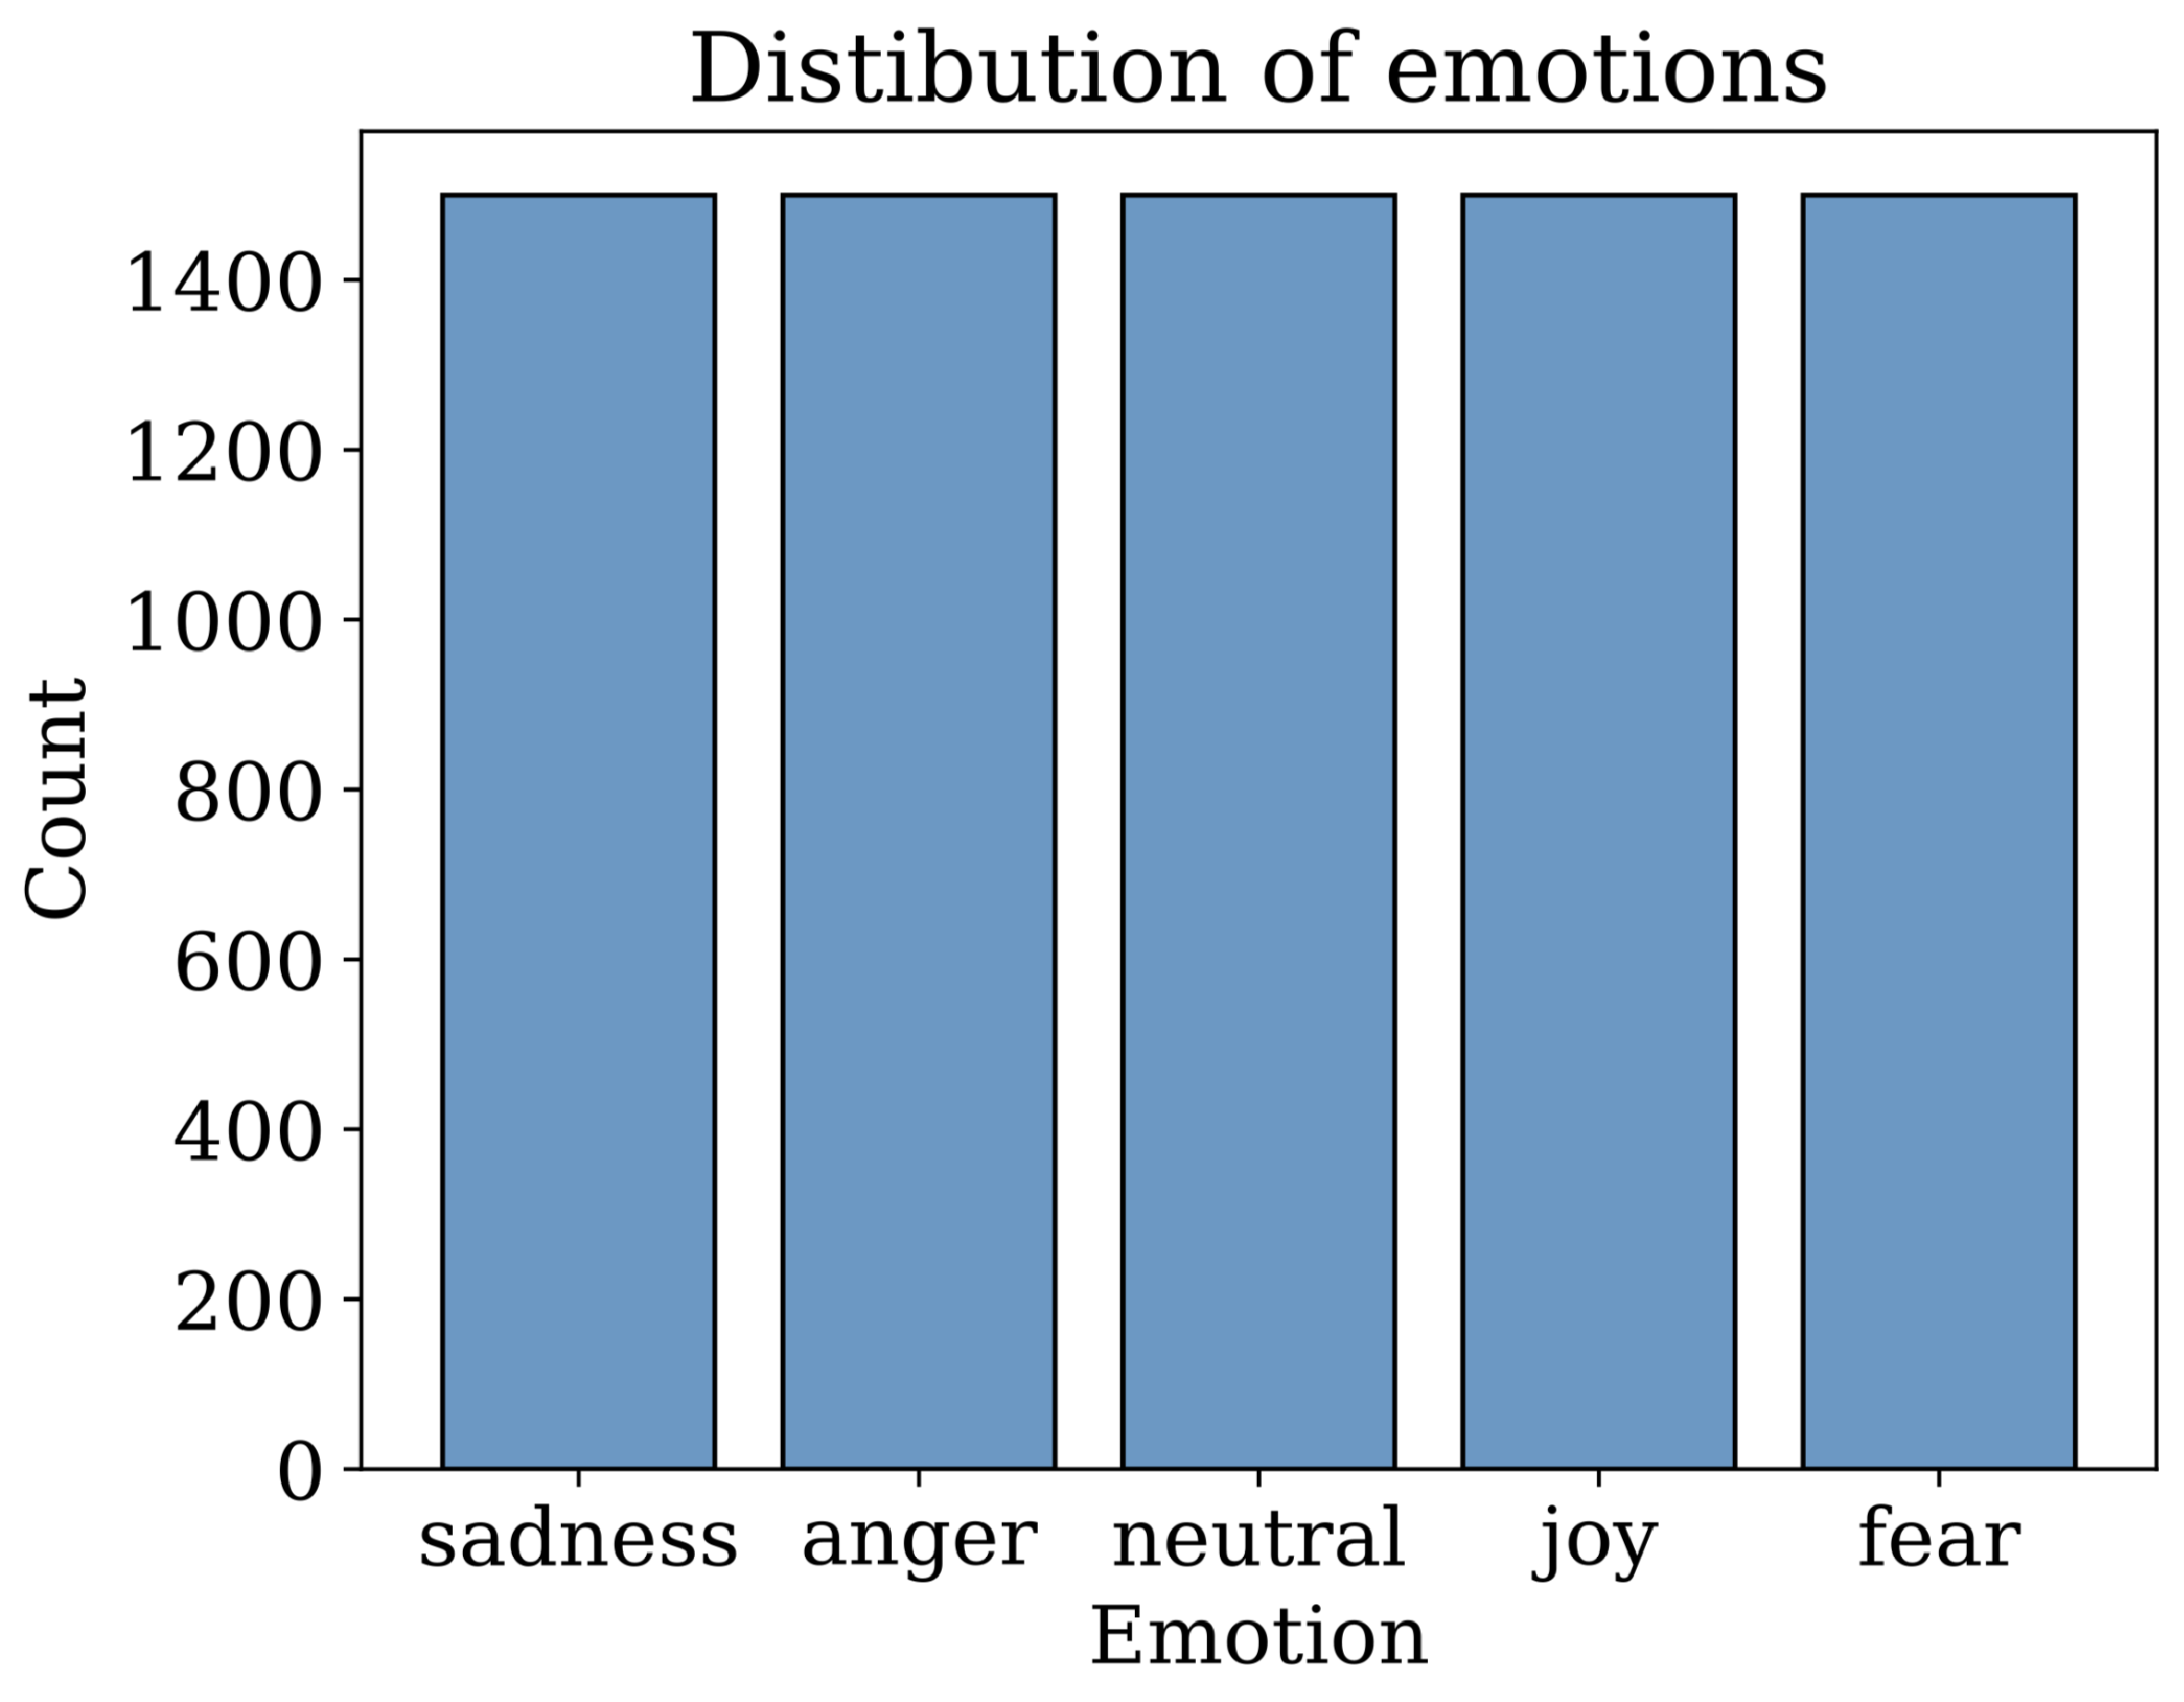
\includegraphics[width=120mm, height=89mm]{/Users/nickpan/courses/msu/sem-7/my-first-project/paper/vis/distr_emot-eps-converted-to.pdf}
	}
	\label{eq:distr_emot}
\end{figure}

\section{Методология}
\subsection{Метрики}
Поскольку используемый датасет сбалансирован по классам, то в качестве основной метрики была взята доля правильных классификаций(accuracy), которая плохо работает в случае дисбаланса классов. Также сравнения велись по точности(Precision), полноте(Recall), F1 мере(F1) с макроусреднением. 

Для каждого класса $y \in Y$:
\begin{itemize}
    \item $TP_y$ -- верные положительные
    \item $FP_y$ -- ложные положительные
    \item $FN_y$ -- ложные отрицательные
\end{itemize}
Точность, полнота и F1 мера с {\bfseries макроусреднением}:
            $$ 
                Precision_{macro} = \frac{1}{|Y|}\sum_{y}\frac{TP_y}{TP_y + FP_y}
            $$
            $$ 
                Recall_{macro} = \frac{1}{|Y|}\sum_{y}\frac{TP_y}{TP_y + FN_y}
            $$
            $$
                F1_{macro} = \frac{2 * Precision_{macro} * Recall_{macro}}
                                  {Precision_{macro} + Recall_{macro}}
            $$
В дальнейшем изложении пометка "macro"\ будет опускаться.
\subsection{Классическое машинное обучение}
\subsubsection{Предобработка текстов}
"Сырые"\ твиты в большинстве своем это "грязные"{}, сильно зашумленные данные. Это сопряжено прежде всего с природой твитов: люди часто пишут сокращениями, с ошибками и прочее. При предобработке текстов использовались стандартные методы в машинном обучении для подготовки текстовых данных на вход алгоритму:
\begin{itemize}
    \item {\bfseries Эмотикон}\\
    Поскольку через текст часто сложно передать эмоции, эмотиконы приобрели очень большую популярность и пользователи нередко используют их в своих твитах. В связи с этим эмотиконы были переведены в текстовый формат с помощью библиотеки Demoji Python, чтобы они помогали в идентификации эмоций в твитах~\cite{wolny}.
    \item {\bfseries Хэштег}\\
    Хэштеги - это фразы без пробелов с префиксом в виде символа решетки (\#), которые часто используются пользователями для упоминания трендовой темы в Твиттере. Все хэштеги были заменены словами без символа решетки. Например, \#hello заменяется на hello. 
    \item{\bfseries Упоминание пользователей}\\
    У каждого пользователя Твиттера есть имя пользователя, связанное с ним. Пользователи часто упоминают других пользователей в своих твитах через @username. В текстах все упоминания пользователей убирались.
    \item{\bfseries URL}\\
    Пользователи часто делятся гиперссылками на другие веб-страницы в своих твитах. Какой-либо конкретный URL-адрес не важен для классификации текста и , если бы ссылки были оставлены, то это привело бы к очень разреженным признакам для текстов причем напрасно. Именно поэтому 
все URL-адреса в твитах были удалены.
    \item{\bfseries Фильтрация стоп-слов и стемминг}\\
    Эмпирически доказано, что фильтрация стоп-слов в наборе данных повышает производительность и скорость вычислений~\cite{saif}, поэтому стоп-слова удалялись. Стемминг также использовался и это еще один метод повышения производительности модели путем сведения производных слов к грамматическому корню, называемому "stem".
\end{itemize}

\subsubsection{Векторизация текстов}

После предобработки тексты векторизовались с помощью наиболее популярного векторного представления -- TF-IDF. Пусть $d$ - документ из коллекции документов $D$, $w_i$ - $i$-е слово из словаря $W$. Мощность (количество элементов) для множеств , как это принято в математике, будем обозначать $|\cdot|$. Тогда векторное представление каждого документа будет выглядеть так:
            $$
            d_{vec} = \begin{pmatrix}
                    tf\!-\!idf( w_1, d, D) \\
                    tf\!-\!idf( w_2, d, D) \\
                    \vdots\\
                    tf\!-\!idf({w_{|W|}}, d, D) \\
                \end{pmatrix},
            $$

            
где $$tf\!-\!idf(w_i, d, D) = \underbrace{tf(w_i, d)}_{term\ frequency} * 
                             \underbrace{idf(w_i, D)}_{inverse\ document\ frequency} =\\$$
                             $$
                             =\underbrace{\frac{\sum_{w' \in d}[w_i = w']\footnotemark}{\sum_{w' \in d}1}}_{tf(w_i, d)} *\ 
                             \underbrace{log\left(\frac{|D|}{\sum_{d \in D}[w_i \in d]}\right)}_{idf(w_i, D)}$$
                             \footnotetext{Используется нотация Айверсона}
Такие веса используются из предположения, что, чем больше документов, в которых встречается слово, тем меньше смысла оно несет в себе и следовательно его вес меньше.
\subsubsection{Модели}
\begin{enumerate}
    \item{\bfseries wKNN} \\
    Вместо классического KNN использовался взвешенный KNN (weighted KNN, wKNN)~\cite{dudani}, в котором веса не равномерно распределены для ближайших соседей объекта, а обратно пропорционально от расстояний от объекта до ближайших соседей. Основными параметрами для этого метрического метода являются: расстояние между текстами и $k$ ближайших соседей.

    В качестве метрики в метрических алгоритмах берут функции убывающие от "близости"{}, поэтому будем отталкиваться именно от "близости"{} текстов. Cогласно Хуанг~\cite{huang}, которая сравнивала различные меры близости для кластеризации текстов, лучшая оказалась косинусная мера:
    $$
    cosine\_similarity(x, y) = \frac{x^{T}y}{\|x\| \|y\|},
    $$ где x, y - векторные представления текстов, а $\|\cdot\|$ - норма вектора. В качестве косинусного расстояния бралась функция:
    $$
    cosine\_distance(x, y) = 1 - cosine\_similarity(x, y)
    $$
    При подборе $k$ можно было воспользоваться эмпирическим правилом и брать $k = \frac{\sqrt{|D|}}{2} = 17$(в нашем случае), однако, поскольку это лишь эмпирическое правило, было решено попробовать перебрать $k$ и оказалось, что лучшим выбором было $k = 52$
    
    \item{\bfseries Logistic Regression} \\
    Логистическая регрессия - это алгоритм машинного обучения с учителем, используемый для задач бинарной или многоклассовой классификации. В контексте машинного обучения он используется для прогнозирования вероятности принадлежности объекта к определенному классу. Существует несколько подходов для использования logistic regression: либо использовать множество бинарных логистических классификаторов и на основе их выдавать ответ (one-vs-one или one-vs-rest) или изменить лосс функцию и на выходе вместо сигмоиды для предсказания вероятностей использовать софтмакс. В данной работе использовался второй подход. Формализуем задачу многоклассовой логистической регрессии. \\
    
     Линейный классификатор при произвольном числе классов $|Y|$   
        $$
        a(x) = \argmax_{y \in Y}\langle w_y, x\rangle,\ x, w_y \in \mathbb{R},
        $$
        где $\langle \cdot, \cdot \rangle$ - скалярное произведение, $w_y$ - веса для метки $y \in Y$.\\
    Вероятность того, что объект $x$ относится к классу $y$:
        $$
        P(y|x, w) = \frac{exp(\langle w_y, x\rangle)}{\sum_{z \in Y}(\langle w_z, x\rangle)} = 
        \softmax_{y \in Y}(\langle w_y, x \rangle)
        $$
    Обучение состоит в максимизации правдоподобия (log-loss) с регулизацией:
    $$
        L(w) = \sum_{i=1}^{l}log(P(y_i|x_i, w) - \frac{\tau}{2}\sum_{y \in Y}\|w_y\|^2 \rightarrow \max_w
    $$
    Для $\tau$ было подобрано значение равное 1.

    \item{\bfseries Multinomial Naive Bayes}\\
    Мультиномиальный байесовский классификатор (Multinomial Naive Bayes Classifier) является разновидностью наивного байесовского классификатора, который использует мультиномиальное распределение для моделирования данных. Этот алгоритм особенно хорошо подходит для решения задач классификации текста и анализа тональности, когда требуется разделить текстовые данные на несколько категорий. Несмотря на то, что классическая теория мультиномиального классификатора предполагает, что на вход подается векторизованные документы по частотам слов в каждом документе, существуют работы, в которых опытным путем было показано, что tf-idf дает лучше результаты~\cite{chingmuankin}. По этой причине в работе был выбран tf-idf для мультиномиального байесовского классификатора.

    \item{\bfseries Support Vector Classifier}\\
    Метод опорных векторов состоит в поиске оптимальной разделяющей гиперплоскости, которая приводит к максимизации ширины разделяющей полосы между классами, следовательно, к более уверенной классификации. SVC работает для бинарной классификации, поэтому в случае мультиклассовой классификации приходится строить несколько алгоритмов SVC и выбирать класс с помощью голосования. В качестве подхода построения таких алгоритмов была выбрана схема one-vs-one, поскольку при использовании one-vs-rest SVC придется обучать на большой выборке данных, что вычислительно менее эффективно, так как на больших данных SVC ресурсоемкий и будет долго обучаться.


    
\end{enumerate}
\subsection{Трансформеры}
\subsubsection{Предобработка и токенизация текстов}
Для всех рассматриваемых версий BERT существуют свои специфичные токенизаторы. Перед подачей в токенизатор предложений\footnote{Под "предложением"\ будем понимать кусок текста, а не синтаксическое предложение} в каждом были убраны ссылки и имена пользователей, поскольку они не несут никакой информации об эмоциях. Несмотря на разницу в токенизаторах, отметим общие принципы: \\
\begin{itemize}
    \item {\itshape Нормализация}, т.е. приведение к нормальному виду, что обычно делается путем приведения слов к нижнему регистру, контролирования специальных символов, в том числе, удаление пробельных символов.
    \item {\itshape Токенизация}, т.е. отображение слов в токены. Для BERT - WordPiece~\cite{yonghui}, для BERTweet и RoBERTa - byte-level BPE(Byte-Pair-Encoding)~\cite{roberta}.
    \item{\itshape Добавление специальных токенов}, такик как '[CLS]', с помощью которого агрегируется информацию о предложении, используемая для задач классификации, а также '[PAD]', '[SEP]', '[EOS]'.   
\end{itemize}

\subsubsection{Модели}
В работе рассмотрены три основные модели: BERT~\cite{devlin}, RoBERTa~\cite{roberta}, BERTweet~\cite{bertweet}, а также их large-аналоги, в которых больше слоев и больше обучаемых параметров. Для решения задачи классификации брался  эмбеддинг, чья размерность 768, который соответствует позиции '[CLS]' токена в токенизированном предложении. Этот эмбеддинг проходил через dropout-слой с вероятностью обнуления элемента равной 0.3, чтобы снизить переобучение, далее через линейный слой и LogSoftMax, поскольку эта функция активации вычислительно более стабильна чем SoftMax (см. Рис. \ref{eq:proposed_model}).
\begin{figure}[h!]
	\caption{\centering Предложенная модель}
	\centering{
	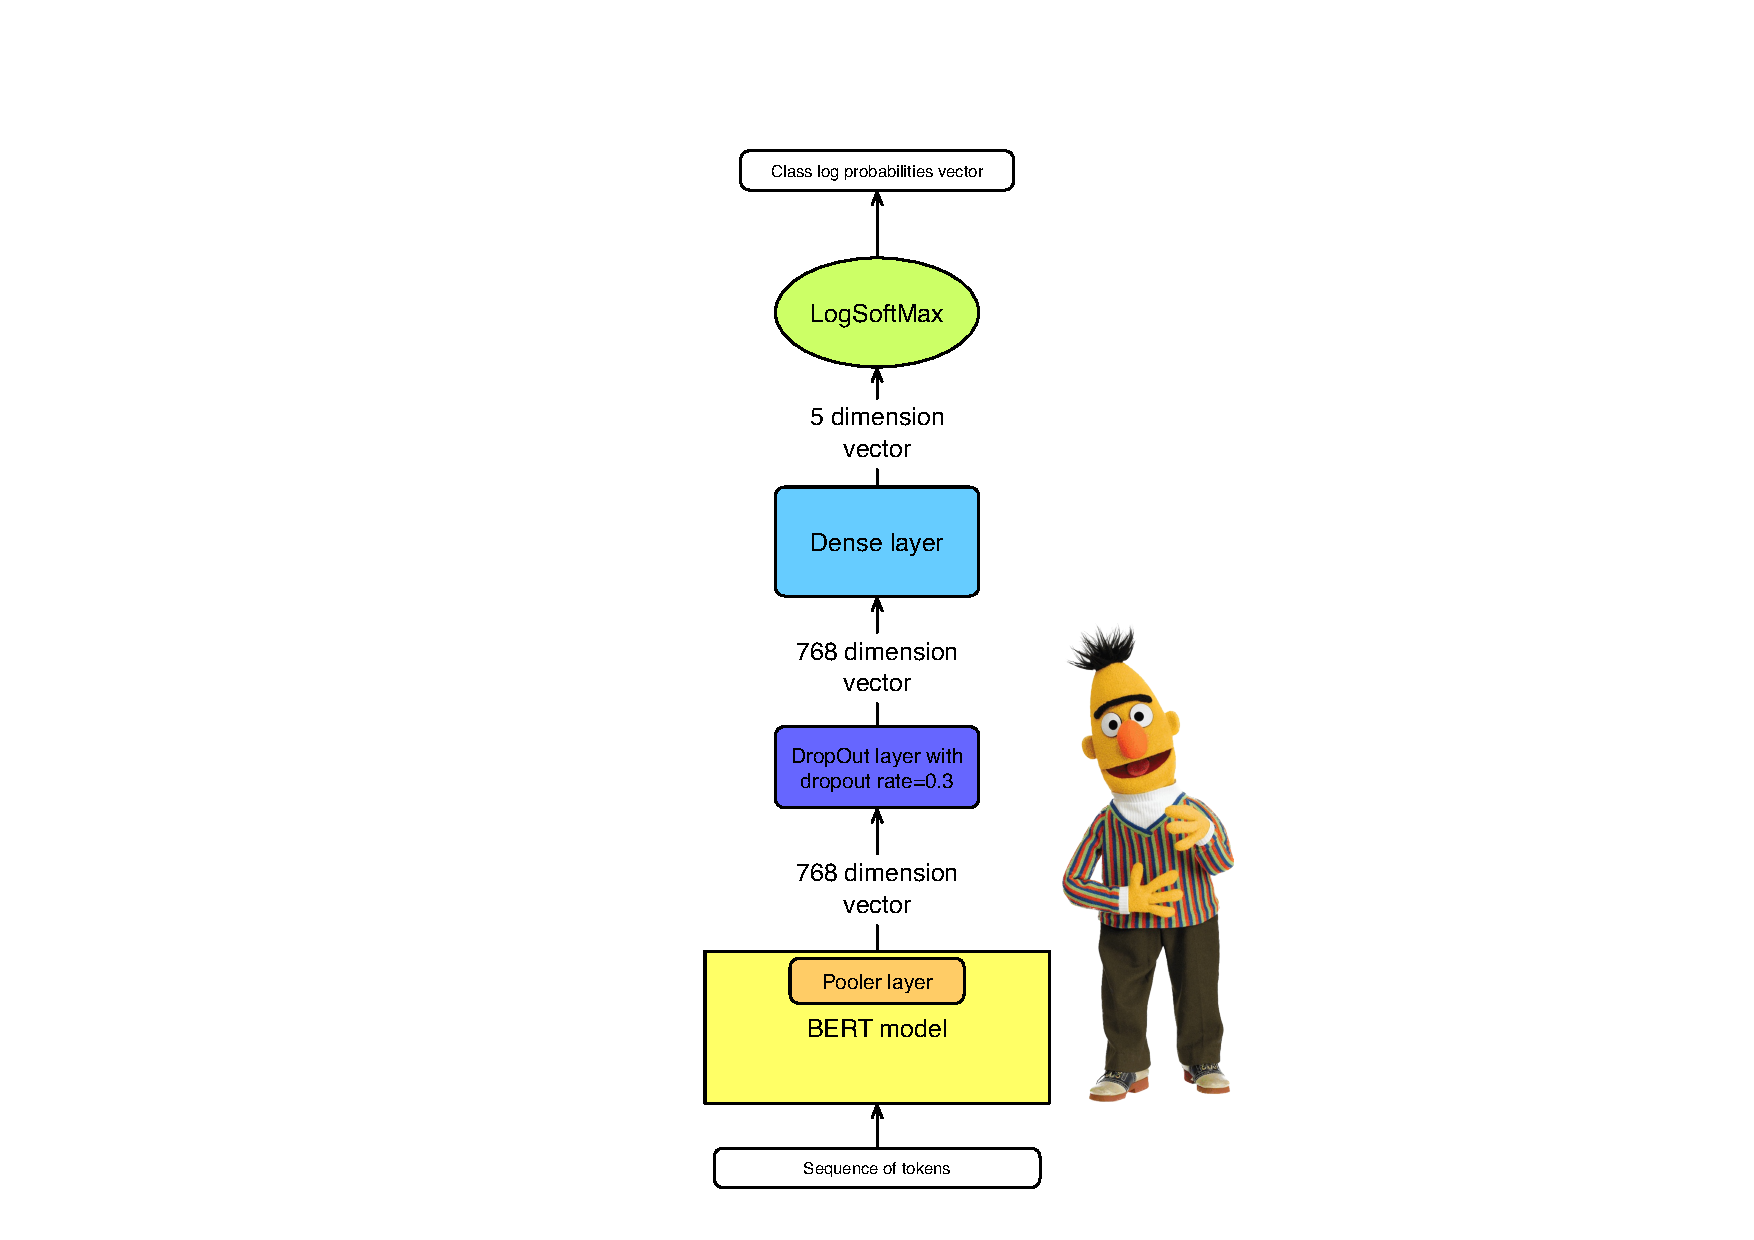
\includegraphics[width=160mm, height=120mm]{/Users/nickpan/courses/msu/sem-7/my-first-project/paper/vis/proposed_model.pdf}
	}
	\label{eq:proposed_model}
\end{figure}
Выбранной функцией потерь была NLLLoss(Negative Log Likelihood loss):
$$
NLLLoss(y) = - log(y)
$$
В качестве оптимизатора был выбран Adam. При обучении использовалось линейное уменьшение шага градиента и  ограничение нормы градиента с максимальной нормой, равной 1, чтобы уменьшить вероятность появления исчезающего или взрывающегося градиента.

\newpage
\bibliographystyle{plain}
\bibliography{references}

\end{document}